\textbf{Musterlösung:Verengtes Rohr}

\begin{figure}[h]
  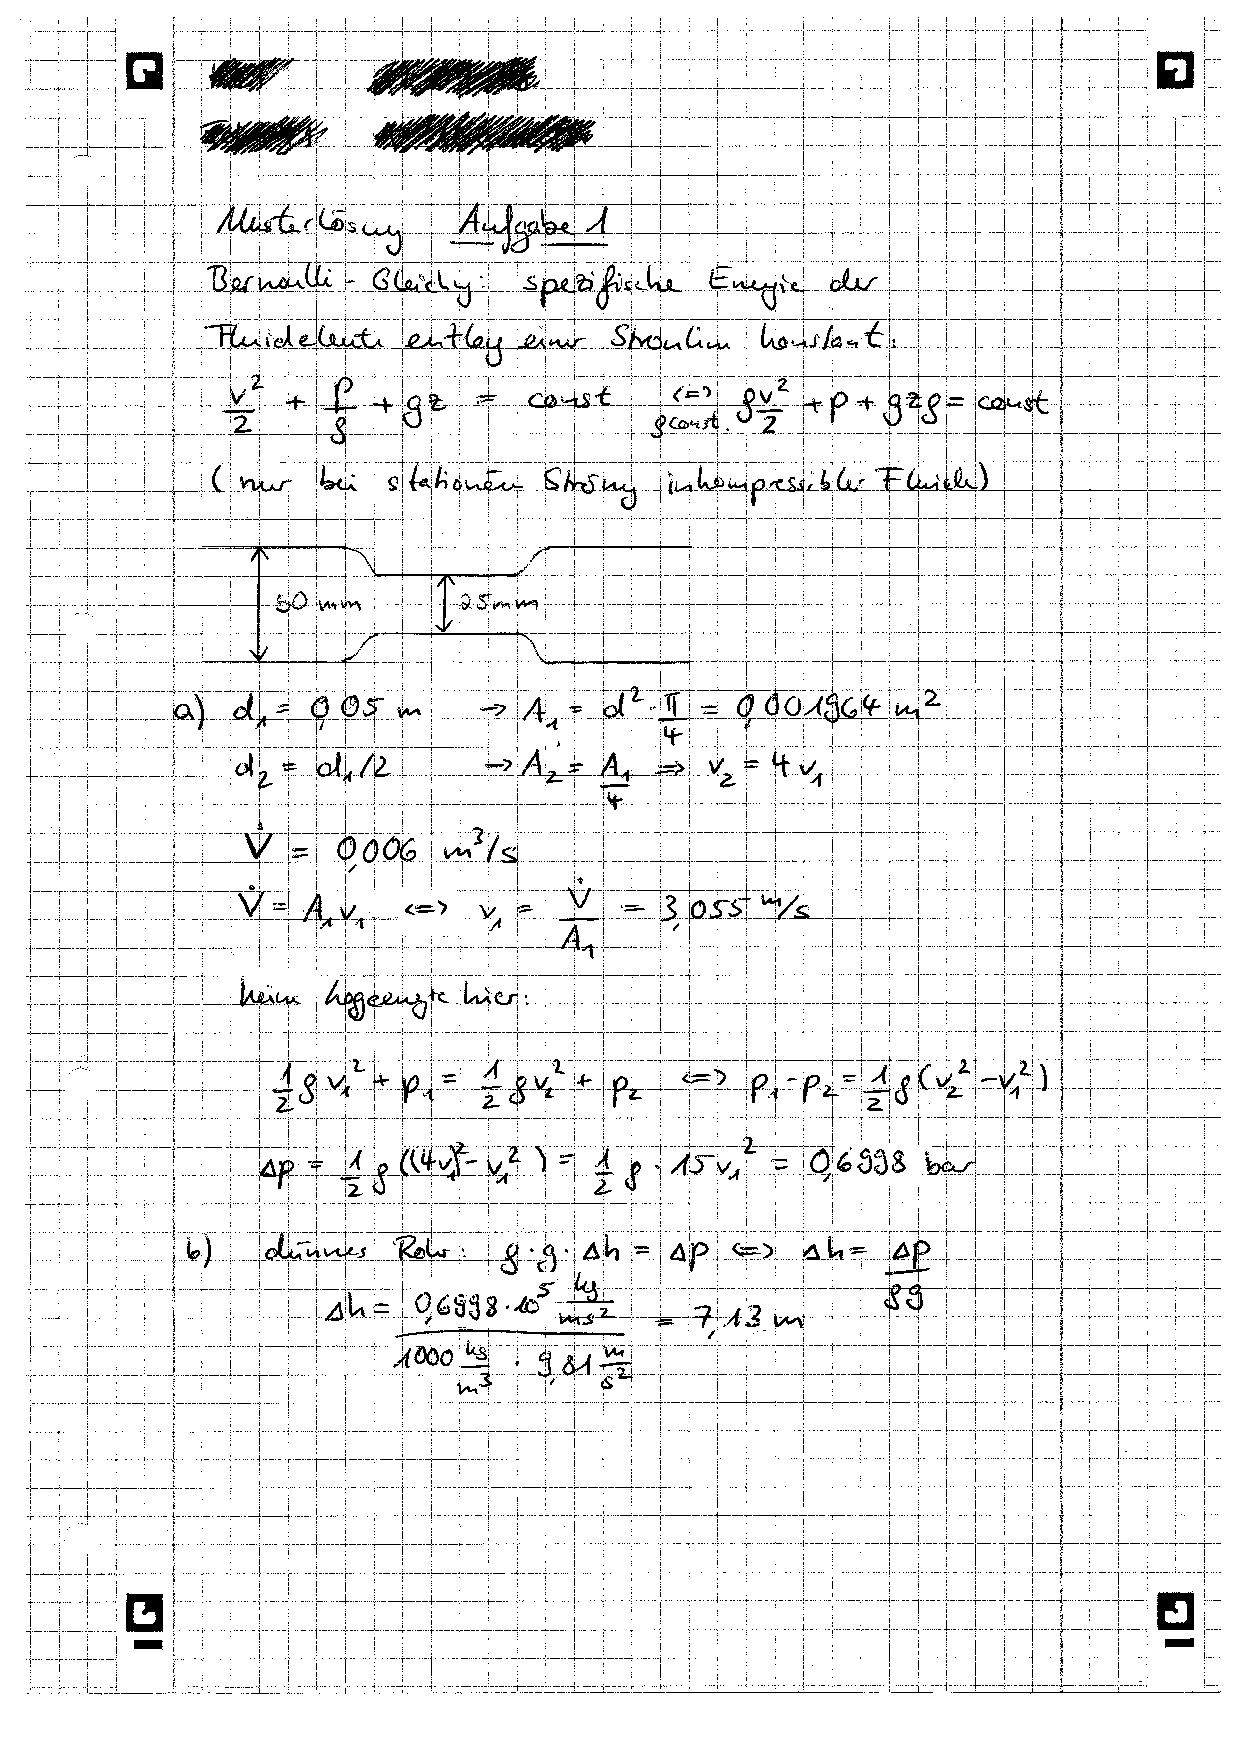
\includegraphics[width = 0.88\textwidth]{Musterlösung/LoesungRohr.pdf}
\end{figure}
\FloatBarrier
\textbf{Musterlösung: Navier-Stokes}

\begin{itemize}
  \item[a.)]
    \begin{align*}
      v_x =& v_y = 0\\
      v_z =& v(r)\\
      \Rightarrow \Delta V =& \frac{1}{r}\frac{\text{d}}{\text{d}r}
      \left(r\frac{\text{d}v}{\text{d}r}\right) = 0
    \end{align*}
  \item[b.)]
    \begin{align*}
      v(r = R_1) =& u\\
      v(r = R_2) =& 0
    \end{align*}
  \item[c.)]
    \begin{align*}
      \frac{\text{d}}{\text{d}r}
      \left(r\frac{\text{d}v}{\text{d}r}\right) = 0\\
      \frac{\text{d}v}{\text{d}r} = \frac{c_1}{r}\\
      \\
      v(r) = c_1\cdot \ln{r} + c_2\\
    \end{align*}
    Jetzt in die Randedingungen einsetzen:
    \begin{align*}
      u = v(R_1) = c_1 \cdot \ln{R_1} + c_2\\
      0 = v(R_2) = c_1 \cdot \ln{R_2} + c_2\\
      \Rightarrow c_1 = \frac{u}{\ln{\frac{R_1}{R_2}}}\qquad
      c_2 = -\frac{u\ln{R_2}}{\ln{\frac{R_1}{R_2}}}
    \end{align*}
    Ergebnis:
    \begin{align*}
      v(r) = u\cdot\frac{\ln{\frac{r}{R_2}}}{\ln{\frac{R_1}{R_2}}}
    \end{align*}
\end{itemize}
\newpage
\textbf{Musterlösung:Zusatzaufgabe}

\begin{figure}[h]
  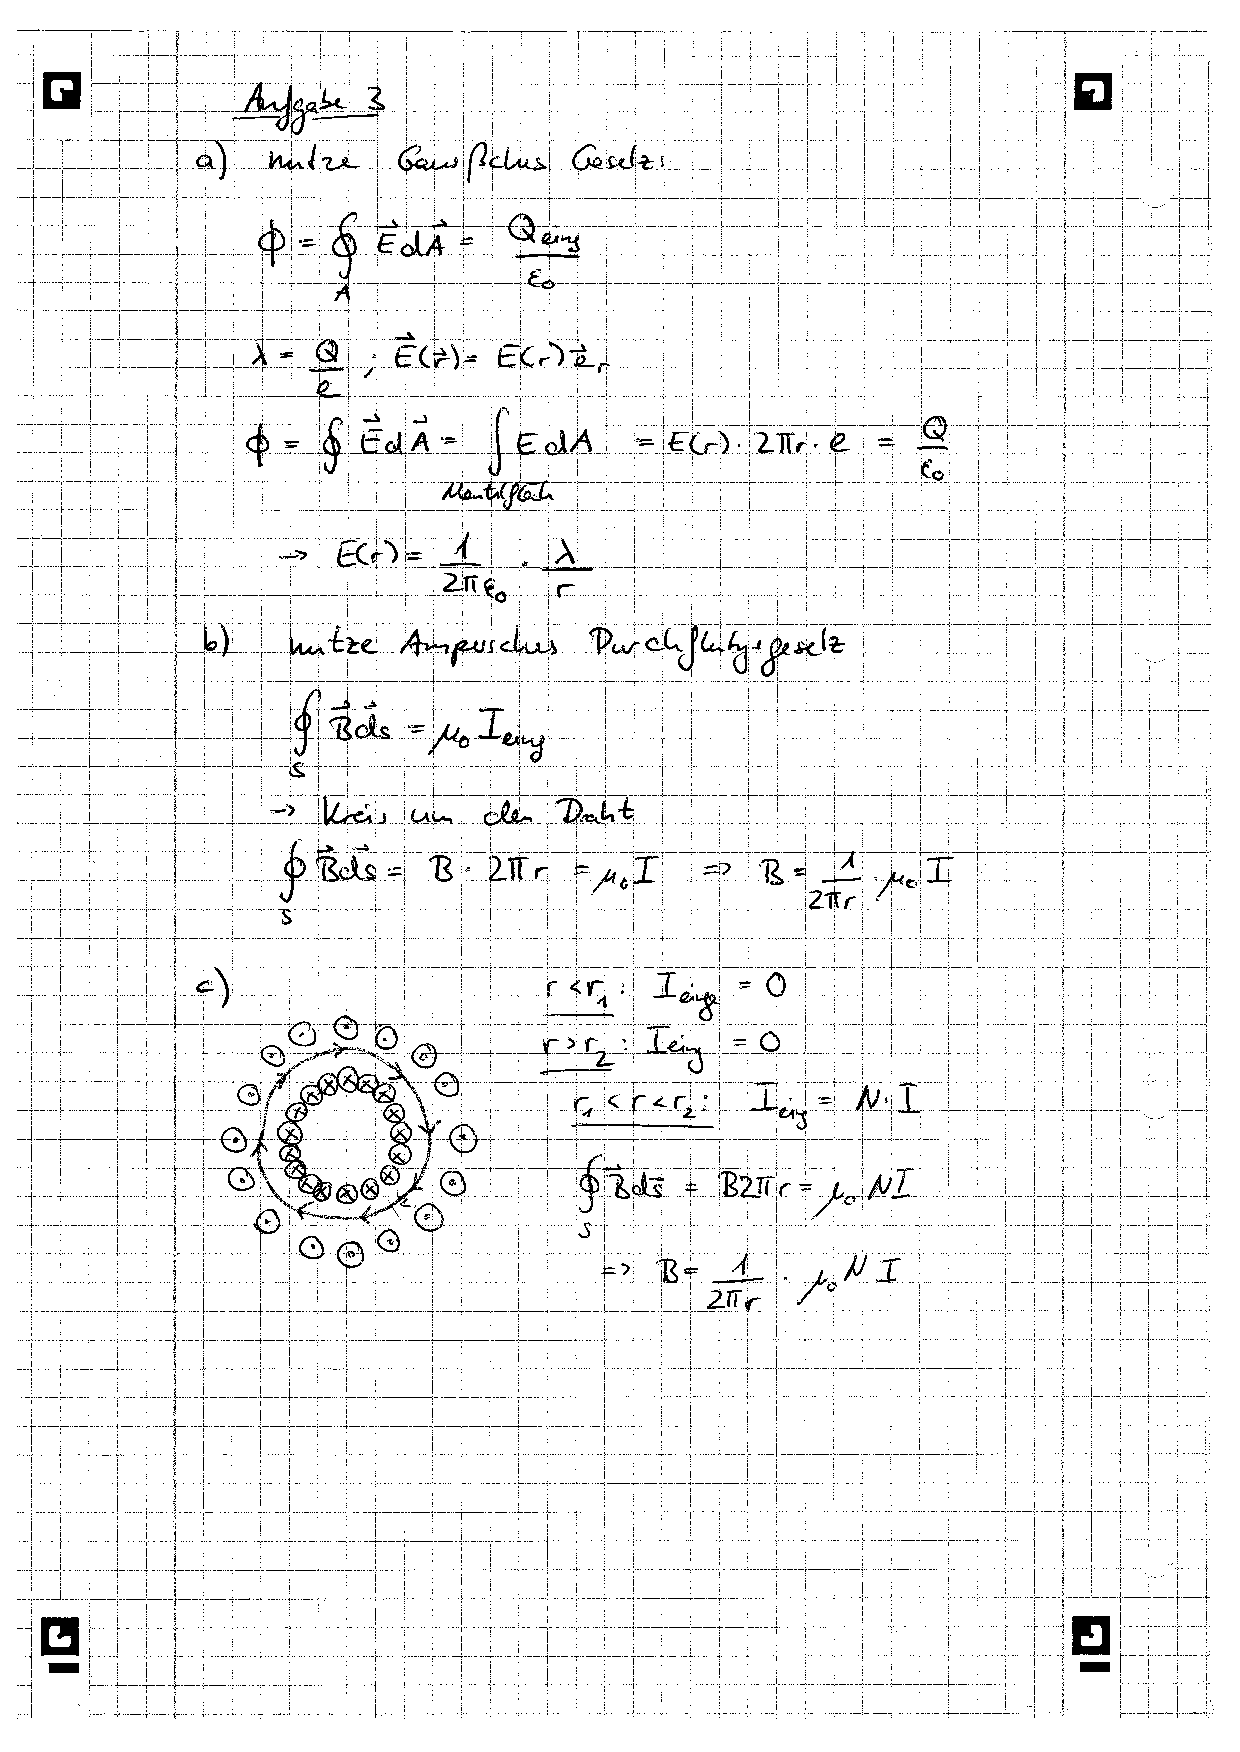
\includegraphics[width = 0.87\textwidth]{Musterlösung/LoesungZusatz.pdf}
\end{figure}
